% Options for packages loaded elsewhere
\PassOptionsToPackage{unicode}{hyperref}
\PassOptionsToPackage{hyphens}{url}
%
\documentclass[
  man,floatsintext]{apa6}
\usepackage{amsmath,amssymb}
\usepackage{iftex}
\ifPDFTeX
  \usepackage[T1]{fontenc}
  \usepackage[utf8]{inputenc}
  \usepackage{textcomp} % provide euro and other symbols
\else % if luatex or xetex
  \usepackage{unicode-math} % this also loads fontspec
  \defaultfontfeatures{Scale=MatchLowercase}
  \defaultfontfeatures[\rmfamily]{Ligatures=TeX,Scale=1}
\fi
\usepackage{lmodern}
\ifPDFTeX\else
  % xetex/luatex font selection
\fi
% Use upquote if available, for straight quotes in verbatim environments
\IfFileExists{upquote.sty}{\usepackage{upquote}}{}
\IfFileExists{microtype.sty}{% use microtype if available
  \usepackage[]{microtype}
  \UseMicrotypeSet[protrusion]{basicmath} % disable protrusion for tt fonts
}{}
\makeatletter
\@ifundefined{KOMAClassName}{% if non-KOMA class
  \IfFileExists{parskip.sty}{%
    \usepackage{parskip}
  }{% else
    \setlength{\parindent}{0pt}
    \setlength{\parskip}{6pt plus 2pt minus 1pt}}
}{% if KOMA class
  \KOMAoptions{parskip=half}}
\makeatother
\usepackage{xcolor}
\usepackage{graphicx}
\makeatletter
\def\maxwidth{\ifdim\Gin@nat@width>\linewidth\linewidth\else\Gin@nat@width\fi}
\def\maxheight{\ifdim\Gin@nat@height>\textheight\textheight\else\Gin@nat@height\fi}
\makeatother
% Scale images if necessary, so that they will not overflow the page
% margins by default, and it is still possible to overwrite the defaults
% using explicit options in \includegraphics[width, height, ...]{}
\setkeys{Gin}{width=\maxwidth,height=\maxheight,keepaspectratio}
% Set default figure placement to htbp
\makeatletter
\def\fps@figure{htbp}
\makeatother
\setlength{\emergencystretch}{3em} % prevent overfull lines
\providecommand{\tightlist}{%
  \setlength{\itemsep}{0pt}\setlength{\parskip}{0pt}}
\setcounter{secnumdepth}{-\maxdimen} % remove section numbering
% Make \paragraph and \subparagraph free-standing
\makeatletter
\ifx\paragraph\undefined\else
  \let\oldparagraph\paragraph
  \renewcommand{\paragraph}{
    \@ifstar
      \xxxParagraphStar
      \xxxParagraphNoStar
  }
  \newcommand{\xxxParagraphStar}[1]{\oldparagraph*{#1}\mbox{}}
  \newcommand{\xxxParagraphNoStar}[1]{\oldparagraph{#1}\mbox{}}
\fi
\ifx\subparagraph\undefined\else
  \let\oldsubparagraph\subparagraph
  \renewcommand{\subparagraph}{
    \@ifstar
      \xxxSubParagraphStar
      \xxxSubParagraphNoStar
  }
  \newcommand{\xxxSubParagraphStar}[1]{\oldsubparagraph*{#1}\mbox{}}
  \newcommand{\xxxSubParagraphNoStar}[1]{\oldsubparagraph{#1}\mbox{}}
\fi
\makeatother
\ifLuaTeX
\usepackage[bidi=basic]{babel}
\else
\usepackage[bidi=default]{babel}
\fi
\babelprovide[main,import]{english}
% get rid of language-specific shorthands (see #6817):
\let\LanguageShortHands\languageshorthands
\def\languageshorthands#1{}
% Manuscript styling
\usepackage{upgreek}
\captionsetup{font=singlespacing,justification=justified}

% Table formatting
\usepackage{longtable}
\usepackage{lscape}
% \usepackage[counterclockwise]{rotating}   % Landscape page setup for large tables
\usepackage{multirow}		% Table styling
\usepackage{tabularx}		% Control Column width
\usepackage[flushleft]{threeparttable}	% Allows for three part tables with a specified notes section
\usepackage{threeparttablex}            % Lets threeparttable work with longtable

% Create new environments so endfloat can handle them
% \newenvironment{ltable}
%   {\begin{landscape}\centering\begin{threeparttable}}
%   {\end{threeparttable}\end{landscape}}
\newenvironment{lltable}{\begin{landscape}\centering\begin{ThreePartTable}}{\end{ThreePartTable}\end{landscape}}

% Enables adjusting longtable caption width to table width
% Solution found at http://golatex.de/longtable-mit-caption-so-breit-wie-die-tabelle-t15767.html
\makeatletter
\newcommand\LastLTentrywidth{1em}
\newlength\longtablewidth
\setlength{\longtablewidth}{1in}
\newcommand{\getlongtablewidth}{\begingroup \ifcsname LT@\roman{LT@tables}\endcsname \global\longtablewidth=0pt \renewcommand{\LT@entry}[2]{\global\advance\longtablewidth by ##2\relax\gdef\LastLTentrywidth{##2}}\@nameuse{LT@\roman{LT@tables}} \fi \endgroup}

% \setlength{\parindent}{0.5in}
% \setlength{\parskip}{0pt plus 0pt minus 0pt}

% Overwrite redefinition of paragraph and subparagraph by the default LaTeX template
% See https://github.com/crsh/papaja/issues/292
\makeatletter
\renewcommand{\paragraph}{\@startsection{paragraph}{4}{\parindent}%
  {0\baselineskip \@plus 0.2ex \@minus 0.2ex}%
  {-1em}%
  {\normalfont\normalsize\bfseries\itshape\typesectitle}}

\renewcommand{\subparagraph}[1]{\@startsection{subparagraph}{5}{1em}%
  {0\baselineskip \@plus 0.2ex \@minus 0.2ex}%
  {-\z@\relax}%
  {\normalfont\normalsize\itshape\hspace{\parindent}{#1}\textit{\addperi}}{\relax}}
\makeatother

\makeatletter
\usepackage{etoolbox}
\patchcmd{\maketitle}
  {\section{\normalfont\normalsize\abstractname}}
  {\section*{\normalfont\normalsize\abstractname}}
  {}{\typeout{Failed to patch abstract.}}
\patchcmd{\maketitle}
  {\section{\protect\normalfont{\@title}}}
  {\section*{\protect\normalfont{\@title}}}
  {}{\typeout{Failed to patch title.}}
\makeatother

\usepackage{xpatch}
\makeatletter
\xapptocmd\appendix
  {\xapptocmd\section
    {\addcontentsline{toc}{section}{\appendixname\ifoneappendix\else~\theappendix\fi: #1}}
    {}{\InnerPatchFailed}%
  }
{}{\PatchFailed}
\makeatother
\keywords{keywords\newline\indent Word count: X}
\usepackage{csquotes}
\ifLuaTeX
  \usepackage{selnolig}  % disable illegal ligatures
\fi
\usepackage{bookmark}
\IfFileExists{xurl.sty}{\usepackage{xurl}}{} % add URL line breaks if available
\urlstyle{same}
\hypersetup{
  pdftitle={Spanish L2 Learners' performance attending to gender grammar cues},
  pdfauthor={Jorge L. Vargas Mutizabal1},
  pdflang={en-EN},
  pdfkeywords={keywords},
  hidelinks,
  pdfcreator={LaTeX via pandoc}}

\title{Spanish L2 Learners' performance attending to gender grammar cues}
\author{Jorge L. Vargas Mutizabal\textsuperscript{1}}
\date{}


\shorttitle{Attending to gender grammar cues}

\authornote{

Correspondence concerning this article should be addressed to Jorge L. Vargas Mutizabal, . E-mail: \href{mailto:jorge.vargas@rutgers.edu}{\nolinkurl{jorge.vargas@rutgers.edu}}

}

\affiliation{\vspace{0.5cm}\textsuperscript{1} Rutgers - The State University of New Jersey\\\textsuperscript{} }

\begin{document}
\maketitle

\section{Data analysis}\label{data-analysis}

\subsection{Reaction times}\label{reaction-times}

In preparation for data analysis, incorrect responses were removed, and the data distribution of reaction times was visually inspected. The long tail of the distribution suggested the presence of outliers, and the Interquartile Range (IQR) method was used to remove them. The difference between the first and third quartiles was computed to obtain the range of the middle 50\% of the distribution. Values that fell below 1.5 x IQR of the Q1 or above 1.5 x IQR of the Q3 were removed. The original data set had 1,343 observations, and 44 observations were removed, keeping 1,299 data points.
A series of nested linear-mixed model comparisons was used to assess the effect of session and conditions (fixed effects) on reaction times, and the random effects were defined as the interaction between the session and condition, item number, and participant. The null model was fitted without fixed effects, while model 1 included session. Then, Model 2 added the session and condition, while Model 3 tested the interaction between them.

\subsection{Accuracy}\label{accuracy}

Similar to reaction times, different models were used to assess how accuracy changed with session and conditions (fixed effect), and the random effects were also the interaction of session and condition, item, and participant. Although logistic regression was used for the binary outcome (correct or incorrect response), the family used was binomial with a logit link function. The null model included accuracy, and the second model included session, while the third model added session and condition. Lastly, the interaction between session and condition was tested in the fourth model.

\section{Results}\label{results}

\subsection{Reaction times}\label{reaction-times-1}

Reaction times for the pretest and posttest decreased across all four conditions: Cond. 1 (2,386 ms to 2,014 ms), for Cond 2 (2,580 ms to 2,143 ms), for Cond 3 (2,471 ms to 2,171 ms), and for Cond 4 (2,439 ms to 2,280 ms). Figure 1.\ref{fig-accuracy} Illustrate the mean reaction times for the two sessions. However, the nested model comparisons (model 1) showed that session did not have a main effect (X²(2) = 3.87, p = 0.14), suggesting that participants' reaction times did not significantly improve in the posttest. Then, adding conditions and session (model 2) showed a main effect (X²(3) = 19.66, p \textless{} .001), suggesting that reaction times in Conditions 2, 3, and 4 significantly varied from Condition 1. Lastly, the interaction between session and condition (model 3) did not show a main effect (X²(6) = 6.99, p = .322), indicating that participants did not significantly improve their reaction times across conditions from the pre to the posttest.

\begin{figure}
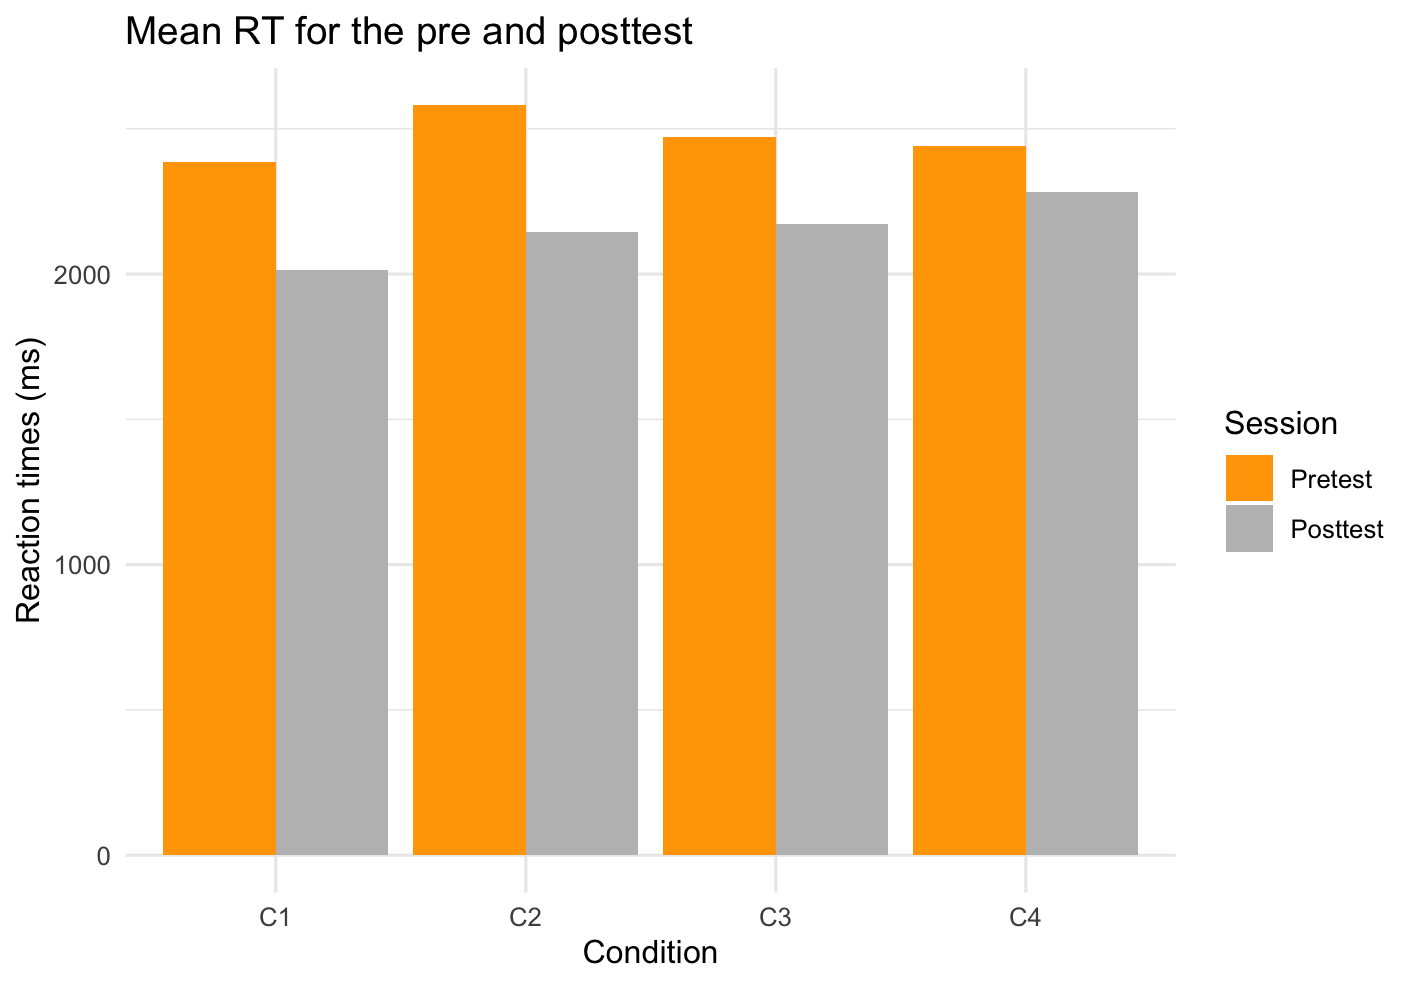
\includegraphics[width=4.72in]{../Plots/RT_plot} \caption{ }\label{fig:unnamed-chunk-1}
\end{figure}

\subsection{Accuracy}\label{accuracy-1}

The mean accuracy also improved across the four conditions between the pre- and posttest. For Cond. 1 (96.5 \% to 97.6 \%), Cond 2 (94.8 \% to 98.2 \%), Cond 3 (93.7 \% to 97.0 \%), and in Cond 4 (72.7 \% to 91.5 \%). Figure 2. Shows the accuracy trends between the two sessions. However, the nested model comparisons did not report a main effect for session (X²(2) = 4.99, p = 0.083), suggesting that participants did not significantly improve across the four conditions. Later, adding session and condition, did not show a main effect for condition, indicating that accuracy did not significantly vary with phrase condition (X²(3) = 5.49, p = 0.139). Lastly, the interaction between session and condition did not report a main effect (X²(6) = 2.82, p = 0.832), which implies that participants did not significantly improve from the pretest to the posttest.

\begin{figure}
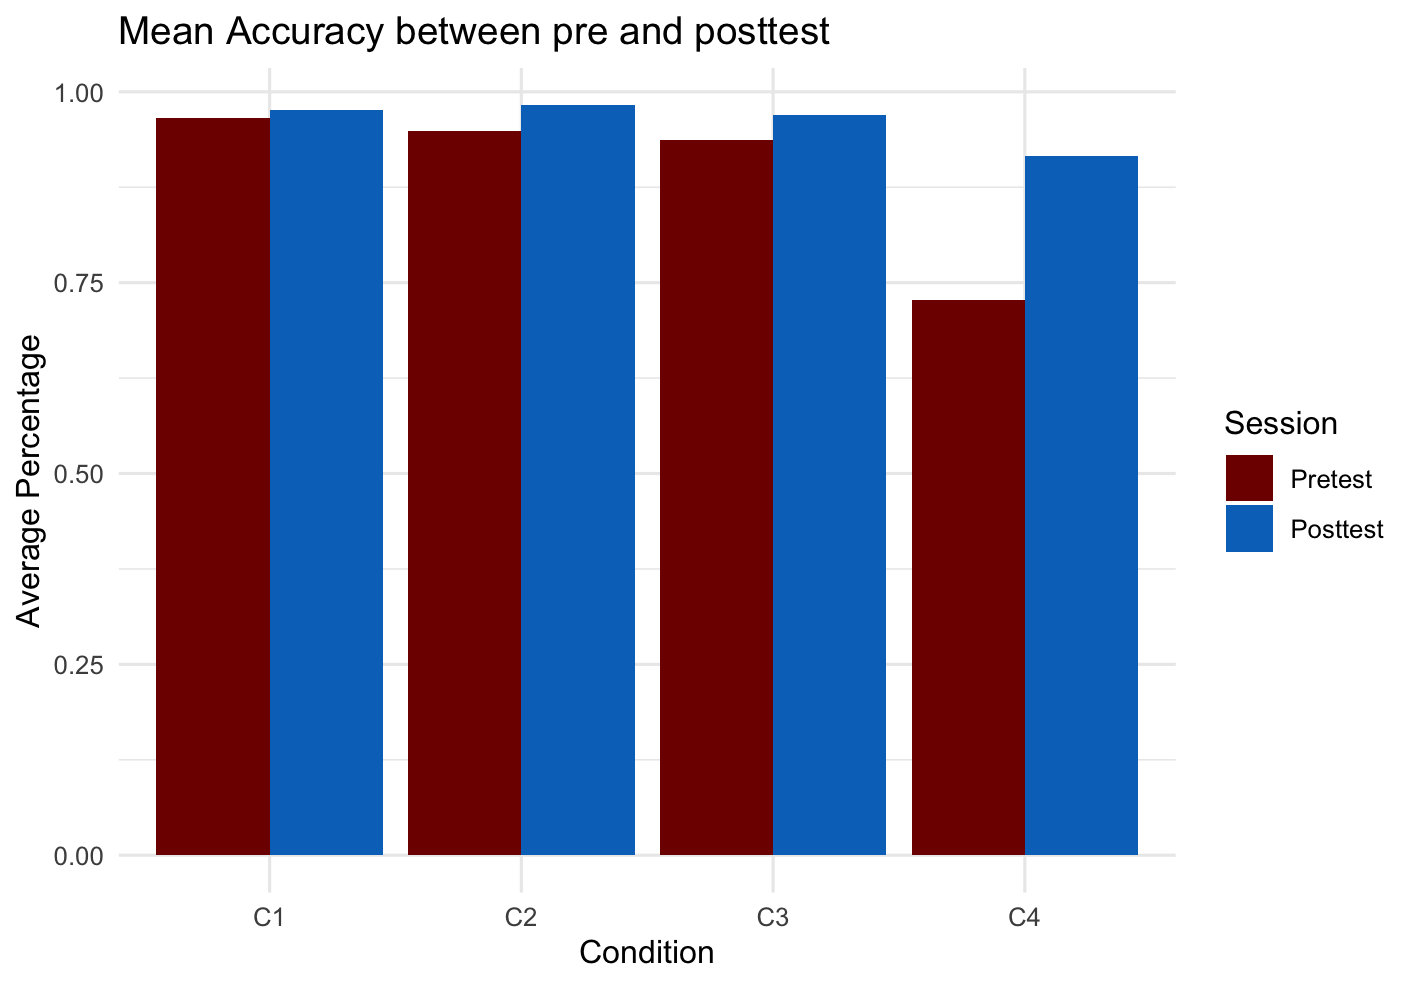
\includegraphics[width=4.72in]{../Plots/Accuracy} \caption{ }\label{fig:unnamed-chunk-2}
\end{figure}


\end{document}
